\documentclass[a4paper]{article}
% The following packages can be found on http:\\www.ctan.org
\usepackage{graphics} % for pdf, bitmapped graphics files
\usepackage[dvips]{graphicx} % for eps
\usepackage{epsfig} % for postscript graphics files
%\usepackage{mathptmx} % assumes new font selection scheme installed
\usepackage{times} % assumes new font selection scheme installed
\usepackage{amsmath} % assumes amsmath package installed
\usepackage{amsthm} % assumes amsmath package installed
%\usepackage{amssymb}  % assumes amsmath package installed
\usepackage{wasysym}
\usepackage{color}
\usepackage{algorithmic}
\usepackage{algorithm}
\usepackage{tensor}
\usepackage{leftidx}
\usepackage{subfigure}
\usepackage{supertabular}
\usepackage{placeins}
\usepackage[cm]{fullpage}
%\renewcommand{\thesubfigure}{\thefigure.\arabic{subfigure}}
%\makeatletter
%\renewcommand{\p@subfigure}{}
%\renewcommand{\@thesubfigure}{\thesubfigure:\hskip\subfiglabelskip}
%\makeatother

%\usepackage[dvips, bookmarks=false, colorlinks=true, pdftitle={Hak-Humanoids2010}]{hyperref}
\newcommand{\mbf}[1]{{\mathbf{#1}}}
\newcommand{\dpartial}[2]{\frac{\partial{#1}}{\partial{#2}}}
\DeclareMathOperator*{\argmin}{arg\,min\,} 

\date{LAAS-CNRS, CNRS-AIST JRL}


\begin{document}

\title{\LARGE Reverse Control for Humanoid Robot Task Recognition}

\author{Sovannara Hak, Nicolas Mansard, Olivier Stasse, Jean Paul Laumond% <-this % stops a space
}

% make the title area
\maketitle

\thispagestyle{empty}
\begin{abstract}
%Statistical approaches are widely used for motion recognition.
%However, those statistical methods need to be applied in a \emph{suitable} space.
Efficient methods to perform motion recognition have been developed
using statistical tools. Those methods rely on primitives learning
in a \emph{suitable space}, for example, the latent space of the joint-angle and/or adequate task spaces.
Learned primitives are often sequential : a motion is segmented according to the time axis.
When working with a humanoid robot, a motion can be decomposed into
parallel sub-tasks. For example, in a waiter scenario,
the robot has to keep some plates horizontal with one of its arms, while placing a plate
on the table with its free hand.
Recognition can thus not be limited to one task per consecutive segment of 
time.
The method presented in this paper
takes advantage of the knowledge of what tasks the robot is able to do and how
the motion is generated from this set of known controllers, to perform a reverse engineering of an
observed motion. This analysis is intended to recognize parallel tasks that
have been used to generate a motion. The method relies
on the task-function formalism and the projection operation into the null space of a task to decouple
the controllers.
The approach is successfully applied on a real robot
to disambiguate motion in different scenarios where two motions look similar but have
different purposes.
\end{abstract}
\vfill
\begin{figure}[h]
  \centering
  \begin{tabular}{cc}
    \includegraphics[height=4.0cm]{img/hrp2Markers.ps} &
    \includegraphics[height=4.0cm]{img/skel.ps} \\
  \end{tabular}
  \caption{HRP-2 robot is equipped with markers. Motions in the joint space are rebuild from a motion capture system.}
  \label{fig:hrp2Markers}
\end{figure}
\vfill
\begin{figure}[h]
  \centering
  \begin{tabular}{cc}
    \includegraphics[width=3.4cm]{img/realRobot/5a/5aFinal1.ps} &
    \includegraphics[width=3.4cm]{img/realRobot/5b/5bFinal1.ps} \\
  \end{tabular}
  \caption{An example of successfull disambiguation: In the picture on the left, HRP-2 is putting its right hand on a 
           desired position while looking at it. On the right, HRP-2 is putting its right hand at the same place while 
           maintaining its chest horizontal.}
  \label{fig:motion5}
\end{figure}
\vfill
\begin{figure}
  \centering
  \includegraphics[height=2.7cm]{img/spotDiff1H.ps}
  \caption{In the picture on the left, HRP2 is grasping a ball in front of him. In the picture on the right HRP2 is both grasping a ball in the front of him and grasping a ball behind him. The motions look very similar. However our method succeeds in disambiguating them (associated videos can be found here: \texttt{http://homepages.laas.fr/shak/videos/}).}
  \label{fig:introExample:graspFeet}
\end{figure}
\vfill
\end{document}


